\documentclass[11pt,a4paper]{article}

\usepackage[margin=1in, paperwidth=8.3in, paperheight=11.7in]{geometry}
\usepackage{amsmath,amsfonts,fancyhdr,bbm,tikz,listings}
\usetikzlibrary{trees}
\usepackage[section,nohyphen]{DomH}
\headertitle{Financial Mathematics - Problem Sheet 8}

\begin{document}

\questionsfalse
% \answersfalse

\title{Financial Mathematics - Problem Sheet 8}
\author{Dom Hutchinson}
\date{\today}
\maketitle

\begin{question}{2.}
  Assume that $\{W_t\}$ is a standard Brownian Motion. The process $\{U_t\}_{t\in[0,1]}$ whose terms are defined by $U_t=W_t-tW_1$ is called a ``Brownian Bridge'' since $U_0=U_1=0$.
\end{question}

\begin{question}{2. a)}
  Show that the covariance between $U_s$ and $U_t$ is given by
  \[ \cov(U_s,U_t)=s(1-t)\text{ for }0\leq s\leq t\leq1 \]
\end{question}

\begin{answer}{2. a)}
  \[\begin{array}{rcl}
    \cov(U_s,U_t)&=&\expect[U_sU_t]-\expect[U_s]\expect[U_t]\\
    &=&\expect[U_sU_t]\\
    &=&\expect[(W_s-sW_1)(W_t-tW_1)]\\
    &=&\expect[W_sW_t]-\expect[sW_1W_t]-\expect[tW_1W_s]+\expect[stW_1^2]\\
    &=&\cov(W_s,W_t)-s\cov(W_1,W_t)-t\cov(W_1,W_s)+st\var(W_1)\\
    &=&s-st-st+st\\
    &=&s(1-t)
  \end{array}\]
\end{answer}

\begin{question}{2. b)}
  Show that the process $\{Y_t\}$ whose terms are defined by $Y_t=(1+t)\cdot U_{t/(1+t)}$ is a Brownian Motion on $[0,\infty)$.
\end{question}

\begin{answer}{2. b)}
  $Y_t$ can be restated as
  \[\begin{array}{rcl}
    Y_t&=&(1+t)U_{t/1+t}\\
    &=&(1+t)\left\{W_{t/1+t}-\frac{t}{1+t}W_1\right\}\\
    &=&(1+t)W_{t/1+t}-tW_1
  \end{array}\]
  For $Y_t$ to be a standard Brownian motion, it must fulfil the following properties
  \begin{enumerate}
    \item \textit{$Y_0=0$}.
    \[\begin{array}{rcl}
      Y_0&=&(1+0)W_{0/1+0}-0W_1\\
      &=&W_0=0
    \end{array}\]
    \item \textit{Increments of $Y_t$ are independent}.
    \par Consider $(Y_t-Y_s)$ with $s\leq t$.
    \[\begin{array}{rcl}
      (Y_t-Y_s)&=&\left\{(1+t)W_{t/1+t}-tW_1\right\}-\left\{(1+s)W_{s/1+s}-sW_1\right\}\\
      &=&(1+s)\left(W_{t/1+t}-W_{s/1+s}\right)-(t-s)\left(W_1-W_{t/1+t}\right)
    \end{array}\]
    Since $W_t$ is standard Brownian motion, the increments $\left(W_{t/1+t}-W_{s/1+s}\right),\left(W_1-W_{t/1+t}\right)$ are independent of $\mathcal{F}_s$ and thus the increment $(Y_t-Y_s)$ is independent of $\mathcal{F}_s$ for all $s\leq t$.
    \item \textit{Increments have stationary Gaussian Distributions}.
    \par As $W_t$ is standard Brownian motion, its increments have gaussian distributions. Thus, by linearity, the increments of $\{Y_t\}$ have gaussian distributions too.
    \par Consider the mean and variance of increment $(Y_t-Y_s)$ with $s\leq t$.
    \[\begin{array}{rcl}
      \expect[Y_t-Y_s]&=&(1+s)\expect\left[W_{t/1+t}-W_{s/1+s}\right]-(t-s)\expect\left[W_1-W_{t/1+t}\right]\\
      &=&0-0=0\\
      \\
      \var[Y_t-Y_s]&=&(1+s)^2\var\left[W_{t/1+t}-W_{s/1+s}\right]-(t-s)^2\var\left[W_1-W_{t/1+t}\right]\\
      &=&(1+s)^2\left(\frac{t}{1+t}-\frac{s}{1+s}\right)-(t-s)^2\left(1-\frac{t}{1+t}\right)\\
      &=&\frac{(1+s)(t-s)}{1+t}-\frac{(t-s)^2}{1+t}\\
      &=&\dots
    \end{array}\]
  \end{enumerate}
  % TODO - I think the variance should become t-s, but it doesn't :()
\end{answer}

\begin{question}{3.}
  Use a computer to approximate and plot sample samples of a standard Brownian Motion. Consider a random walk $\{S_j\}_{j\in\nats}$ defined by $S_0=0,\ S_n=S_{n-1}+X_n$ where $X_1,X_2,\dots\iid N(0,1)$.
  \par Remember that the process $\{S_t^n\}_{t\in[0,1]}$ is derived by setting $S_t^n=S_j/\sqrt{n}$ for every $t=j/n$ and linear interpolation in between, approximates the Brownian Motion on $[0,1]$ if $n$ is large.
\end{question}

\begin{question}{3. a)}
  Use $n=1000$ and make a plot of two realisations of your approximation to Brownian Motion.
\end{question}

\begin{answer}{3. a)}
\end{answer}
  I wrote the following python code
  \begin{lstlisting}[language=Python]
    import numpy as np
    from scipy import stats
    import matplotlib.pyplot as plt

    def sample_standard_norm():
        return stats.norm(0,1).rvs(1)[0]

    def standard_brownian_motion(n:int):
        X_is=[sample_standard_norm() for _ in range(1,n)]
        S_ns=[0]+list(np.cumsum(X_is))
        W_ts=[x/np.sqrt(n) for x in S_ns]
        return W_ts

    n=1000
    for i in range(2):
        plt.plot([x/n for x in range(n)],standard_brownian_motion(n))
    plt.show()
  \end{lstlisting}
  Which produced this plot
  \begin{center}
    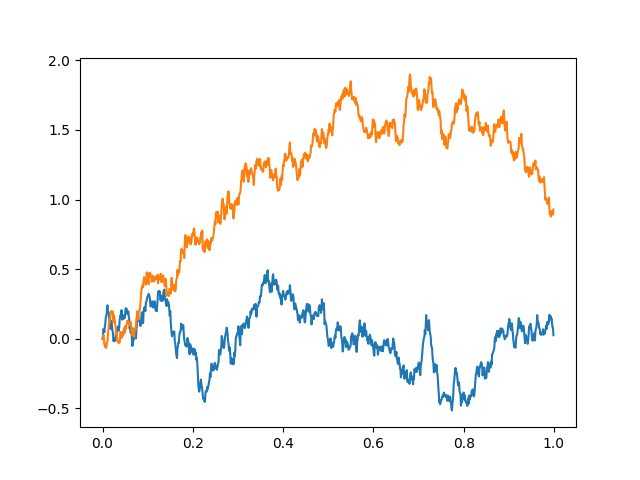
\includegraphics[width=.7\textwidth]{img/3_a.png}
  \end{center}

\begin{question}{3. b)}
  Finally add a drift term to the Brownian Motion $W_t+\mu t$. Again, use $n=1000$ and make a plot of a realisation of this process for $\mu=-3$ and $\mu=30$.
\end{question}

\begin{answer}{3. b)}
\end{answer}
  I extended the code above
  \begin{lstlisting}[language=Python]
    def drift_brownian_motion(n:int,mu:float):
        W_ts=standard_brownian_motion(n)
        W_ts_drift=[W_ts[t]+mu*t for t in range(n)]
        return W_ts_drift

    n=1000

    plt.plot([x/n for x in range(n)],drift_brownian_motion(n,-3))
    plt.plot([x/n for x in range(n)],drift_brownian_motion(n,30))
    plt.show()
  \end{lstlisting}
  Which produced this plot
  \begin{center}
    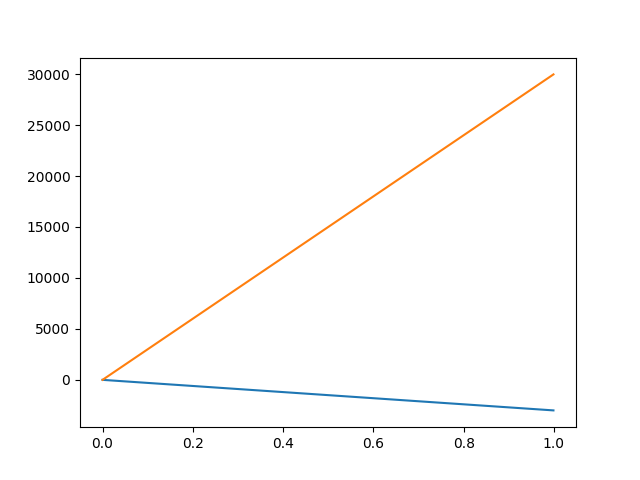
\includegraphics[width=.7\textwidth]{img/3_b.png}
  \end{center}

\end{document}
